\chapter{Other malware}

\section{Hajime}

\section{Goldoon}

\section{BotenaGo}

Identified in November 2021 by AT\&T Alien Labs researchers, BotenaGo is a backdoor that provides cybercriminals access to devices through 33 exploit functions. Their first analysis was performed by reverse engineering the malware's binary and it revealed that the malware associates each exploit function with a string that represents a potential target system, similar to a signature. This is needed because the malware sends a ``GET'' request to the target and then searches into the returned data for the signature. For example the string ``\texttt{Server: Boa/0.93.15}'' is mapped to the function \texttt{main\_infectFunctionGponFiber} which exploit the CVE-2020-8958 vulnerability. They also privide a search result on Shodan that shows 2 milion potential targets. This number decreased in the years as you can see in \Cref{fig:boa-shodan}. All the exploits can be found in \Cref{fig:all-vulnerabilities-botenago} which illustrates the \texttt{scannerInitExploit} from its source code.

\begin{figure}[ht]
    \centering
    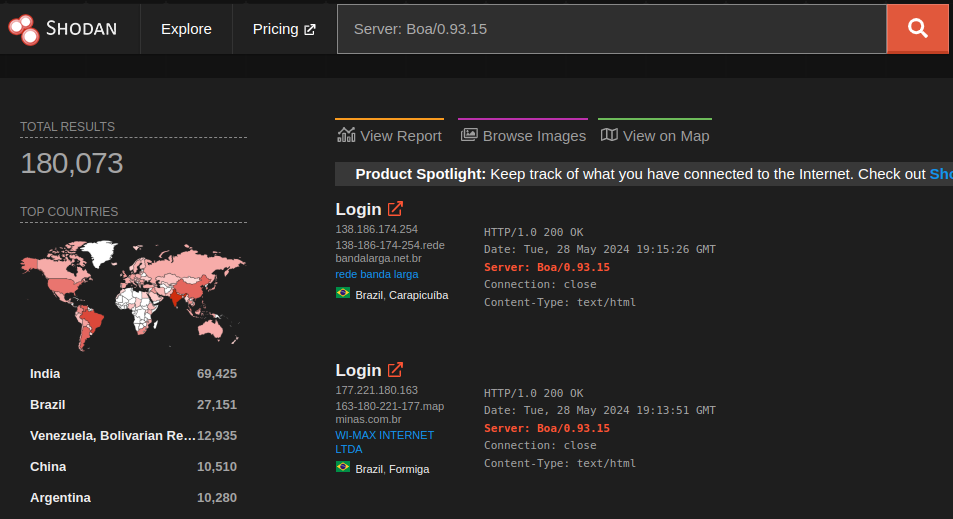
\includegraphics[scale=0.4]{resources/images/boa-shodan.png}
    \caption{Shodan search result for Boa/0.93.15}
    \label{fig:boa-shodan}
\end{figure}

The CNC has two ways of sending command to the infected device:

\begin{enumerate}
    \item Use one of the two backdoor ports (31412 and 19412) to send a command to the device. On port 19412, it lissens for the victim IP address and once received it tries each exploit on that IP.
    \item It listens on a system IO user input. For example it can be accessed locally by using telnet. 
\end{enumerate}

In 2022 its source code was leaked on GitHub and AT\&T Alien Labs provided another analysis which did not provide new information but confirmed the previous analysis. \cite{att-botenago-reverse,att-botenago-sourcecode}

\begin{figure}[ht]
    \centering
    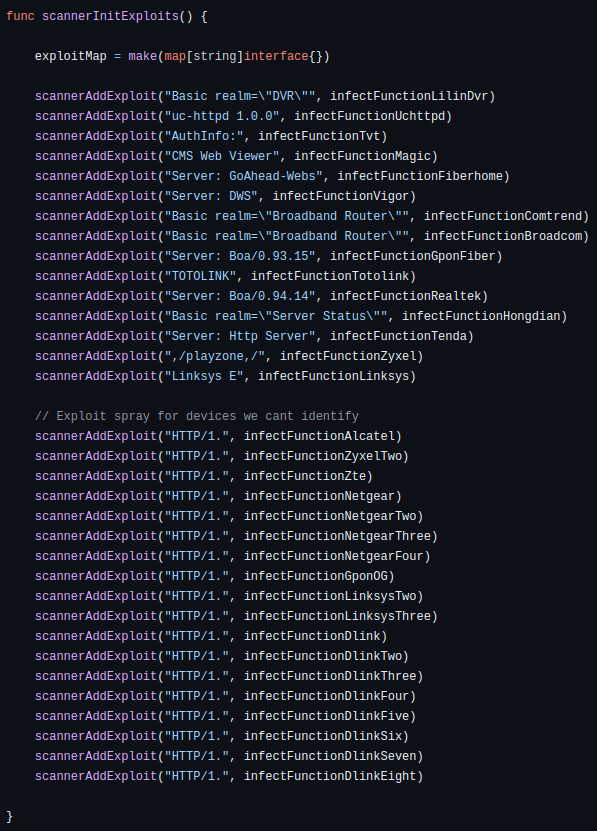
\includegraphics[scale=0.5]{resources/images/all-vulnerabilities-botenago.png}
    \caption{All the vulnerabilities exploited by BotenaGo}
    \label{fig:all-vulnerabilities-botenago}
\end{figure}

\section{Malware comparison}

